\section{Object Recognition\buch{Ch. 12}}
\begin{itemize}
\item Recognition of \emph{individual} image regions called \emph{object} or \emph{pattern}
\item Concept of ``learning'' from sample patterns
\end{itemize}

\subsection{Patterns and Pattern Classes\buch{Ch. 12.1}}
\begin{itemize}
	\item A \emph{pattern} is an arrangement of descriptors
		(as in \ref{sec:representationDescription}) in pattern classification
		called \emph{features}.
	\item A \emph{pattern class} is a set of patterns, denoted $\omega_1, \omega_2, ..., \omega_W$ W is the number of classes
	\item The goal is to assign a given patter into a class
\end{itemize}

\subsubsection{Vectors}
\begin{itemize}
	\item Used for quantitative descriptors
	\item every dimension contains the numerical value of a descriptor
	\item $x =
		\begin{bmatrix}
			x_1 \\
			x_2 \\
			\vdots \\
			x_n \\
		\end{bmatrix}$
\end{itemize}
Example: Classifying flowers based on petal length and width into one of three
classes.

\subsubsection{Strings}
Structural information can be captured in strings. Example
\nameref{sec:boundaryDescriptors}
\begin{itemize}
	\item Connectivity patterns (order is important)
	\item Compact description, better than sampling into a feature vector
\end{itemize}

\subsubsection{Tree}
If there is hierarchy then a descriptor which is based on a tree structure
should be used.

% TODO: Tikz Tree einfügen

\subsection{Recognition Based on Decision Theory\buch{Ch. 12.2}}
\paragraph{Discriminant functions}
The core of decision theory $d_i(x)$ defined for each class $\omega_i$.
These are not known and finding them is the main goal.

A class $\omega_i$ is selected if
\begin{align*}
d_i(x) > d_j(x) && j=1,2, \cdots, W; j \neq i
\end{align*}
The interesting parts are decision boundaries between classes
\begin{align*}
	d_i(x) - d_j(x) = 0
\end{align*}

\subsubsection{Matching\buchSeite{866}}
Each class is represented by prototypes.
A vector $x$ belongs to the class with the shortest distance.
% TODO: Tikz Diagramm mit klassen, prototypen und grenzen
\paragraph{Minimum distance classifier}
The mean vector of a class is a powerful prototype vector.
\begin{align*}
	m_j = \frac{1}{N_j} \sum_{x\in \omega_j}x_j && j = 1,2,\dots, W
\end{align*}
A simple matching function is the Euclidean distance.
\begin{align*}
	D_i(x) = ||x-m_j|| = \left(x^Tm_j\right)^{1/2}
\end{align*}
The resulting discriminant function which is the largest, when the distance is
the smallest.
\begin{align*}
	d_j(x) = x^Tm_j - \frac{1}{2}m_j^Tm_j
\end{align*}
The decision boundary between class $\omega_i$ and $\omega_j$ will be
\begin{align*}
	d_{ij}(x) &= d_i(x) - d_j(x)\\
	&= x^t(m_i-m_j) - \frac{1}{2}(m_i-m_j)^T(m_i+m_j) = 0
\end{align*}
Which is a line through the midpoint of $m_i$ and $m_j$ for $n=2$.
For $n=3$ its a plane and for $n>3$ it's a hyperplane.
% TODO: Tikz mit diagram
% TODO: Evt. Beispiel?

\paragraph{Matching by correlation\buchSeite{869}}
Calculate cross-correlation between a mask $w(x,y)$ of size $m$ $n$ and an image
$f(x,y)$ to find the mask in the image.
\begin{align*}
	c(c,y) = \sum_s\sum_tw(s,t)f(x+s,y+t)
\end{align*}
This is sensitive to contrast and average intensity in $f$ and $w$.
Hence the normalized cross correlation is used
\begin{align*}
	\gamma(x,y) = \frac{\sum_s\sum_t\left[w(s,t)-\bar{w}\right]\left[f(x+s,y+t)-\bar f_{xy}\right]}
	{
	\left\lbrace
		\sum_s\sum_t\left[w(s,t)-\bar w\right]^2
		\sum_s\sum_t\left[f(x+s,y+t)-\bar f_{xy}\right]^2
	\right\rbrace^{\frac{1}{2}}
	}
\end{align*}
$y(x,y)$ is always in range $[-1, 1]$, where +1 is perfect match and -1 a perfect anti-match.
This is sensitive to scale and rotation.

\subsubsection{Optimum Statistical Classifiers\buchSeite{872}}
A classifier which results in the lowest average risk of incorrect classification.
\paragraph{Foundation}
% TODO: komplettieren


\subsubsection{Neural Networks\buchSeite{882}}

Class of algorithms which find decision functions directly by training.

\paragraph{Perceptron for two pattern classes}

The perceptron learns a linear decision function that separates two linearly separable training sets.

\begin{figure}[htb]
\centering
\begin{tikzpicture}[font=\tiny
]
	\tikzstyle{entry} = [circle, draw, inner sep=0, fill=black]
	\tikzstyle{line} = [draw, -latex']
	\tikzstyle{line node} = [rectangle, fill=white]
	\newcommand{\m}{0.5}

	\node (sum) at (1.5,-3*\m) [draw,circle]{$\Sigma$};
	\foreach \x/\xtext in {1, 2, 3.5/i, 5/n, 6/n+1} {
		\node[entry] (in\xtext) at (0,-\x*\m){};
            \if \x6
				\node[left]at (in\xtext){$1$};
            \else
				\node[left]at (in\xtext){$x_{\xtext}$};
            \fi
		\path[line] (in\xtext) -- node[line node]{$w_{\xtext}$}+(1,0) -- (sum);
	}

	\draw[loosely dotted] (in2) -- (ini) --(inn);

	\node (out) at (2.5,-3*\m) [draw,inner sep=7]{};

	\draw (out.west) --  +(0.4,0);
	\draw (out.south west) ++(0.1,0.1) -- ++(0.1,0) -- ++(0,0.3) -- ++(0.15,0);

	\path[line] (sum) -> (out);
\end{tikzpicture}

\caption{Perceptron model for two pattern classes}
\label{fig:perceptron}
\end{figure}
\begin{align*}
d(x) = \sum_{i=1}^nw_ix_i + w_{n+1}
\end{align*}

The function which maps the weighted sum of the input to the output is called \emph{activation function}.
In \ref{fig:perceptron} a sign function is used.
For multilayer NN a sigmoid (\ref{fig:sigmoid}) is common.

The constant input of 1 gives the offset.
A convenient notation is the augmented pattern vector:

\begin{align*}
y_i &= x_i & i=1,2,\dots,n \\
y_{n+1} &= 1 \\
d(y) &= \sum_{i=1}^{n+1}w_iy_i = w^Ty \\
\end{align*}

\paragraph{Training algorithms\buchSeite{886}}
Train the weights of the perceptron so that it can distinguish between classed, using training sets.
For linear separable classes, a simple, iterative algorithm is:
\begin{itemize}
\item
Pattern vectors of the training set are presented repetitively, the weight vector is changed if a misclassification happens.
\item The training stops, when there are no more misclassifications.
\end{itemize}

for $d(y)>0 \rightarrow \omega_1$ and $d(y)<0 \rightarrow \omega_2$

\begin{align*}
\text{if } y(k) \in \omega_1 \text{ and } w^T(k)y(k) \leq 0 && \rightarrow && w(k+1) = w(k) +cy(k) \\
\text{if } y(k) \in \omega_2 \text{ and } w^T(k)y(k) \geq 0 && \rightarrow && w(k+1) = w(k)-cy(k)
\end{align*}


$c$ is a positive correction increment.
This algorithm converges in a finite number of steps for linearly separable training data.

This is not possible for nonseparable classes.
Hence minimizing the squared error is the target.

\begin{align*}
J(w) = \frac{1}{2}(r-w^Ty)^2
&& r \text{ is the desired response}
\end{align*}

To minimize this we use the delta correction algorithm
\begin{align*}
\Delta w &= \alpha e(k)y(k) \\
\Delta w &= w(k+1)-w(k) && \text{weighting change} \\
e(k) &= r(k) - w^T(k)y(k) && \text{error}
\end{align*}

The change of the error becomes
\begin{align*}
\Delta e &= -\alpha e(k) y^T(k) y(k) \\
 &= - \alpha e(k) ||y(k)||^2
\end{align*}

So $\alpha$ controls the speed of error reduction.
For stability $\alpha$ must be smaller than 2.
In practice $\alpha$ is picked below 1.

\paragraph{Multilayer feedforward neural networks\buchSeite{889}}
These allow for multiclass pattern recognition, also for non linear separable classes.
They are stacked banks of perceptrons with the sigmoid as activation function (\ref{fig:sigmoid}).

\begin{figure}[htp]
\centering
\begin{tikzpicture}
	\tikzstyle{entry} = [circle, draw, inner sep=1, fill=black]
	\tikzstyle{perz} = [circle, draw, inner sep=10]
	\tikzstyle{line} = [draw, -latex']
	\newcommand{\xstr}{2}
	\newcommand{\ystr}{2}

	% entries
	\foreach \y/\yt in {1, 2, 3, 5/n} {
		\node[entry] (n0\y)  at (0,-\y*\ystr){};
		\node[left] at (n0\y){$x_{\yt}$};
	}

	% network
	\foreach \x in {1,2,3} {
		\foreach \y in {1,2,3,5} {
			\node[perz] (n\x\y) at(\x*\xstr,-\y*\ystr) {};
		}
	}

	% connections
	\foreach \na/\nb in {0/1,1/2,2/3} {
		\foreach \j in { 1, 2,3,5} {
			\foreach \i in {1,2,3,5} {
				\draw (n\na\j) -- (n\nb\i);
			}
		}
	}

	% text
	\foreach \x in {0,1,2,3} {
		\node[] at(\x*\xstr,-4*\ystr) {$\vdots$};
	}
	\node[] at(4*\xstr,-3.5*\ystr) {$\vdots$};


	%output
	\foreach \y/\yt in {2/1,3/2, 5/W} {
		\node[perz] (n4\y)  at (4*\xstr,-\y*\ystr+0.5*\ystr){};
		\node[right] (end) at (5*\xstr,-\y*\ystr+0.5*\ystr){Class $\omega_\yt$};
		\path[line] (n4\y) -- (end);
		\foreach \yb in {1,2,3,5} {
			\draw (n3\yb) -- (n4\y);
		}
	}

	\foreach \x/\xt/\xtt in {1/J,2/K,3/P,4/Q/Q = W} {
		\node[below,text width=1.7cm] at(n\x5.south) {Layer \xt{} $N_\xtt$ nodes};
	}
\end{tikzpicture}

\caption{Multilayer feed forward network}
\end{figure}

\begin{figure}[htp]
\centering
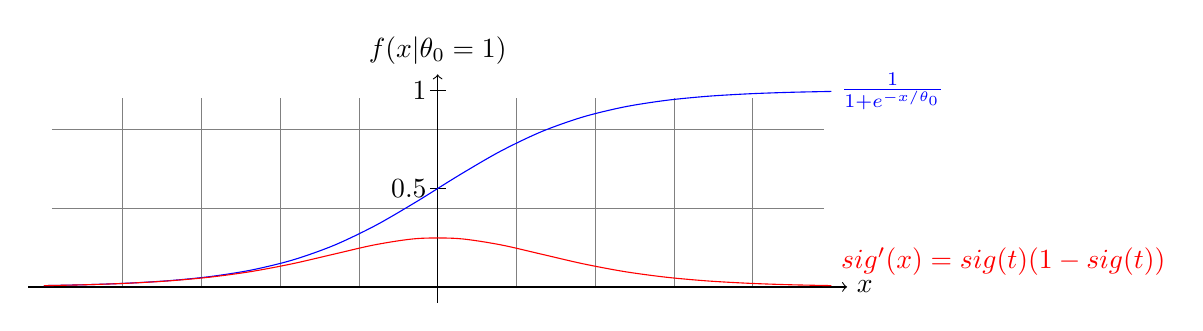
\begin{tikzpicture}[domain=-5:5, smooth, samples=20]
	\draw[very thin, color=gray] (-4.9,0.0) grid (4.9,2.4);

	\draw[->] (-5.2,0) -- (5.2,0) node[right] {$x$};
	\draw[->] (0,-0.2) -- (0,2.7) node[above] {$f(x|\theta_0=1)$};
	\draw (-0.1,2.5) --(0.1,2.5) node [left] {$1~$};
	\draw (-0.1,1.25) -- (0.1,1.25) node [left] {$0.5~$};

	\draw[color=blue] plot (\x,{2.5 / (1+exp(-\x))}) node[right] {$\frac{1}{1+e^{-x/\theta_0}}$};
	\draw[color=red]  plot (\x,{2.5 / (1+exp(-\x)) * (1-1/(1+exp(-\x)))}) node[above right] {$sig'(x)=sig(t)(1-sig(t))$};
\end{tikzpicture}


\caption{Sigmoid function}
\label{fig:sigmoid}
\end{figure}

If $K$ is the layer preceding layer $J$ then the input to the activation function of node $j$ in layer $J$ is the weighted sum of the outputs of Layer $K$.

\begin{align*}
I_j = \sum_{k=1}^{N_k}w_{jk}O_k
\end{align*}

\paragraph{Training by back propagation}
\begin{itemize}
\item A training vector is presented at
the input and the desired response
at the output
\item For all nodes, the input and output values are calculated
\item Starting at the output layer, the
deltas are calculated and back
propagated
\item Now the weights are updated
\end{itemize}

\begin{align*}
\Delta w_{jk} &= \alpha \delta_j O_k& \\
\delta_j &= (r_j-O_j) h'_j(I_j) & \text{if layer $J$ is the output Layer} \\
\delta_j &= h'_j(I_j) \sum_{p=1}^{N_p}\delta_p w_{jp} & \text{if layer $J$ is an internal layer and layer $P$ is the next layer}
\end{align*}

Since $sig'(t) = sig(t)(1-sig(t))$ for $\theta_0=1$ the derivative of the activation function becomes
\begin{align*}
h'_j(I_j) = O_j(1-O_j)
\end{align*}

\paragraph{Some facts about NN}
\begin{itemize}
\item Training with noisy data helps improving performance
\item Training with more patterns also
\item Single layer perceptron results in hyperplanes
\item Two layers result in open or closed convex regions
\item Three layers result in arbitrary (limited by the number of nodes) regions
\item More than three layers are never needed
\end{itemize}

\subsection{Structural Methods\buch{Ch. 12.3}}

